%!TEX program = xelatex


\documentclass[aspectratio=169]{beamer}
%\documentclass{beamer}

\usepackage{blindtext}

\usepackage{beamerthemeFeecBUT}

\usepackage{xltxtra}
\usepackage[export]{adjustbox}

\usepackage{amssymb}% http://ctan.org/pkg/amssymb
\usepackage{pifont}% http://ctan.org/pkg/pifont
\newcommand{\cmark}{\ding{51}}%
\newcommand{\xmark}{\ding{55}}%
% \usepackage[paperwidth=29cm, paperheight=15cm]{geometry}
% \usepackage[a5paper, landscape]{geometry}

\defaultfontfeatures{Ligatures=TeX}

\def\checkmark{\tikz\fill[scale=0.4](0,.35) -- (.25,0) -- (1,.7) -- (.25,.15) -- cycle;}

\title{Nástroje pro diagnostiku integrity souborového systému v OS Linux}
\subtitle{Obhajoba diplomové práce}
\author{Bc. Vojtěch Vladyka}
\garant{Ing. Petr Petyovský, Ph.D.}
\date{6.června 2017}

\begin{document}
	\addtolength{\textwidth}{-20pt}
	\addtolength{\textheight}{-20pt}
  \frame{\titlepage}
   
  \begin{frame}
% TODO predelat podle skutecnosti
    \frametitle{Obsah}
	\vspace{40 pt}
	\begin{enumerate}
	  \Large\item Úvod
	  \\ \textcolor{ExecusharesGrey}{\footnotesize\hspace{1em}\large Cíl práce a nástroje kontroly integrity.}	
	  \Large\item Universal Disk Format
	  \\ \textcolor{ExecusharesGrey}{\footnotesize\hspace{1em}\large Co to je UDF?}
	  \Large\item UDF Filesystem Consistency Check
	  \\ \textcolor{ExecusharesGrey}{\footnotesize\hspace{1em}\large Návrh a realizace samotného nástroje.}
	  \Large\item Výsledky
	  \\ \textcolor{ExecusharesGrey}{\footnotesize\hspace{1em}\large Ukázka výsledků práce.}
	  \Large\item Závěr
	  \\ \textcolor{ExecusharesGrey}{\footnotesize\hspace{1em}\large Shrnutí výsledků práce.}
	\end{enumerate}
	\end{frame}

	\section{Úvod}
		\begin{frame}
			\frametitle{Cíl práce}
			\vspace{40 pt}
            \center
			\huge Cílem práce je vytvořit nástroje pro~diagnostiku integrity dat souborových systémů v~OS~Linux, pro~které v~současnosti tato podpora neexistuje.
		\end{frame}
        \begin{frame}
            \frametitle{Nástroje kontroly integrity dat}
            % TODO popsat fsck nástroje a jejich existenci pro FS v Linuxu
            \begin{itemize}
                \Large\item Nástoj \texttt{fsck} kontroluje metadata a žurnály souborových systémů v~GNU/Linux.
                \Large\item Pro každý souborový systém je tento nástroj \textit{jiný} (obvykle je dodáván s nástroji k souborovému systému.)
                \Large\item Integrita samotných dat je zajištěna médiem samotným (ECC~bloky)
            \end{itemize}
        \end{frame}
        \begin{frame}
            \frametitle{Volba souborového systému}
            % TODO popsat důvody výběru UDF
            \vspace{30pt}
            \huge
            \center
            Při rešerši bylo zjištěno,\\že pro souborový systém \textit{Universal~Disk~Format} tyto nástroje \textbf{chybí}.

            \vspace{30pt} 
            \Large
            Vzhledem k univerzálnosti a perspektivě tohoto souborového systému byl \textbf{vybrán pro další práci}.
        \end{frame}

	\section{Universal Disk Format}
		\begin{frame}
			\frametitle{Co to je?}
            \vspace{40pt}
            \huge
            Universal Disk Format (UDF) je:
            \begin{itemize}
                \Large\item souborový systém navržený původně pro optická média,
                \Large\item náhrada zastaralého souborového systému ISO~9660,
                \Large\item vhodný pro přenos dat mezi různými operačními systémy,
                \Large\item multiplatformní od návrhu,
                \Large\item podporovaný v GNU/Linux do verze 2.01 pro zápis (nejnovější verze je 2.60 pouze pro čtení.)
%
%                \Large\item První verze vznikla v roce 1995, poslední vydaná (2.60) je~z~roku~2005
%                \Large\item Linux umí číst/zapisovat na všechny verze, ale vytvářet jen~do~verze~2.01~(rok 2000)
            \end{itemize}
            UDF není:
            \begin{itemize}
                \Large\item vhodný jako systémový disk,
                \Large\item žurnálovaný.
            \end{itemize}
        \end{frame}
		\begin{frame}
			\frametitle{Multiplatformnost UDF}
			\vspace{40 pt}
			\center
            \begin{figure}
			    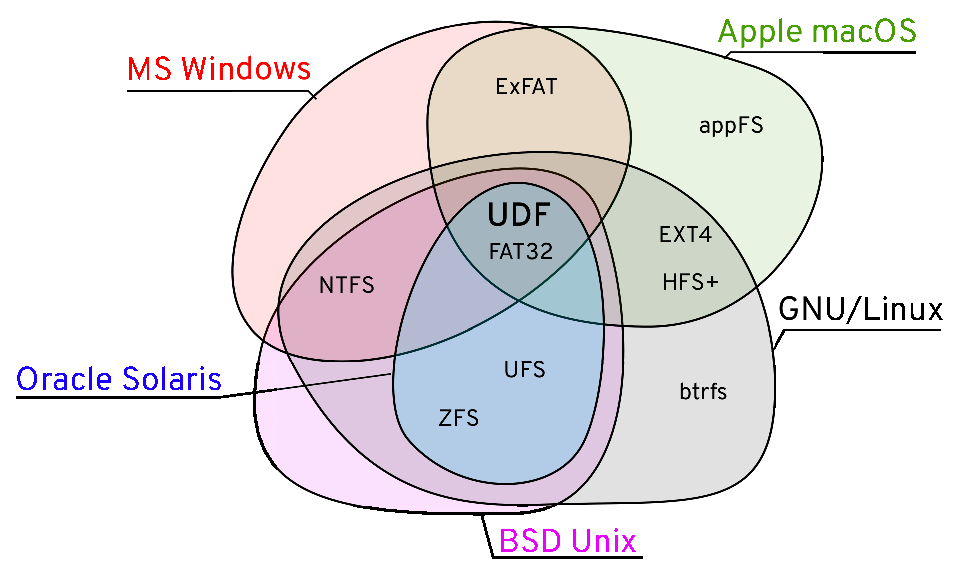
\includegraphics[width=10.2cm]{udf-podpora.eps}
            \end{figure}
		\end{frame}
        \begin{frame}
            \frametitle{Deskriptory UDF}
            % TODO popsat deskriptory a jejich zabezpeceni a chyby
			\vspace{40 pt}
			\center
            \begin{figure}
			    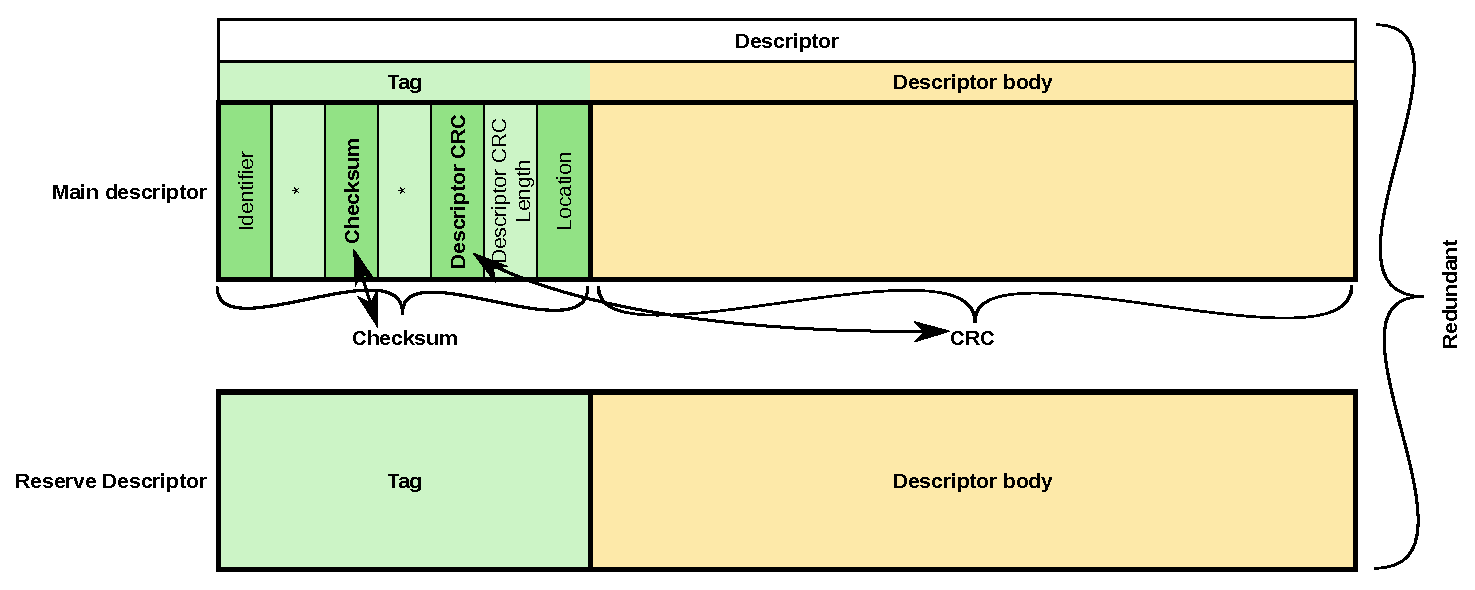
\includegraphics[width=14.5cm]{det-ch.eps}
            \end{figure}
        \end{frame}
		\begin{frame}
			\frametitle{Struktura UDF}
			\vspace{40 pt}
			\center
            \begin{figure}
			    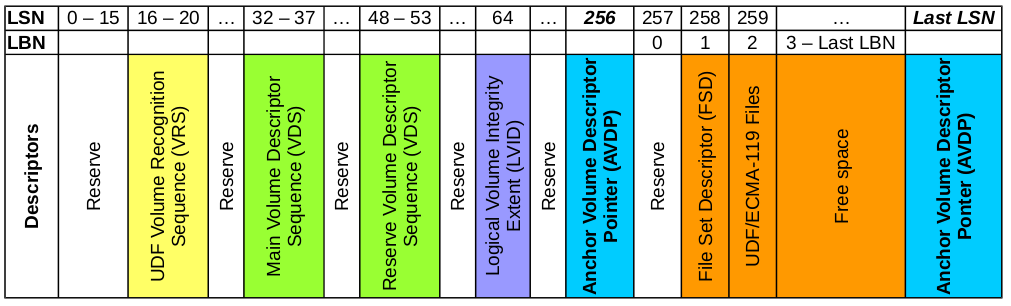
\includegraphics[width=14cm]{UDF-example-schema.png}
                \caption{\Large{Ukázka struktury UDF}}
            \end{figure}
		\end{frame}
	
    \section{UDF Filesystem Consistency Check}
        \begin{frame}
            \frametitle{Cíl nástroje}
            \vspace{30pt}
            \begin{itemize}
                \huge\item Detekovat poruchy na souborovém systému UDF.
                \huge\item Pokud to je možné, poruchy opravit.
                \huge\item Podpora až do standardu UDF 2.01.
                \huge\item Být \textbf{první open source řešení}.
            \end{itemize}
        \end{frame}
        \begin{frame}
            \frametitle{Navržená struktura nástroje}
            %TODO obrazek s ramecky...
			\vspace{30 pt}
			\center
            \begin{figure}
			    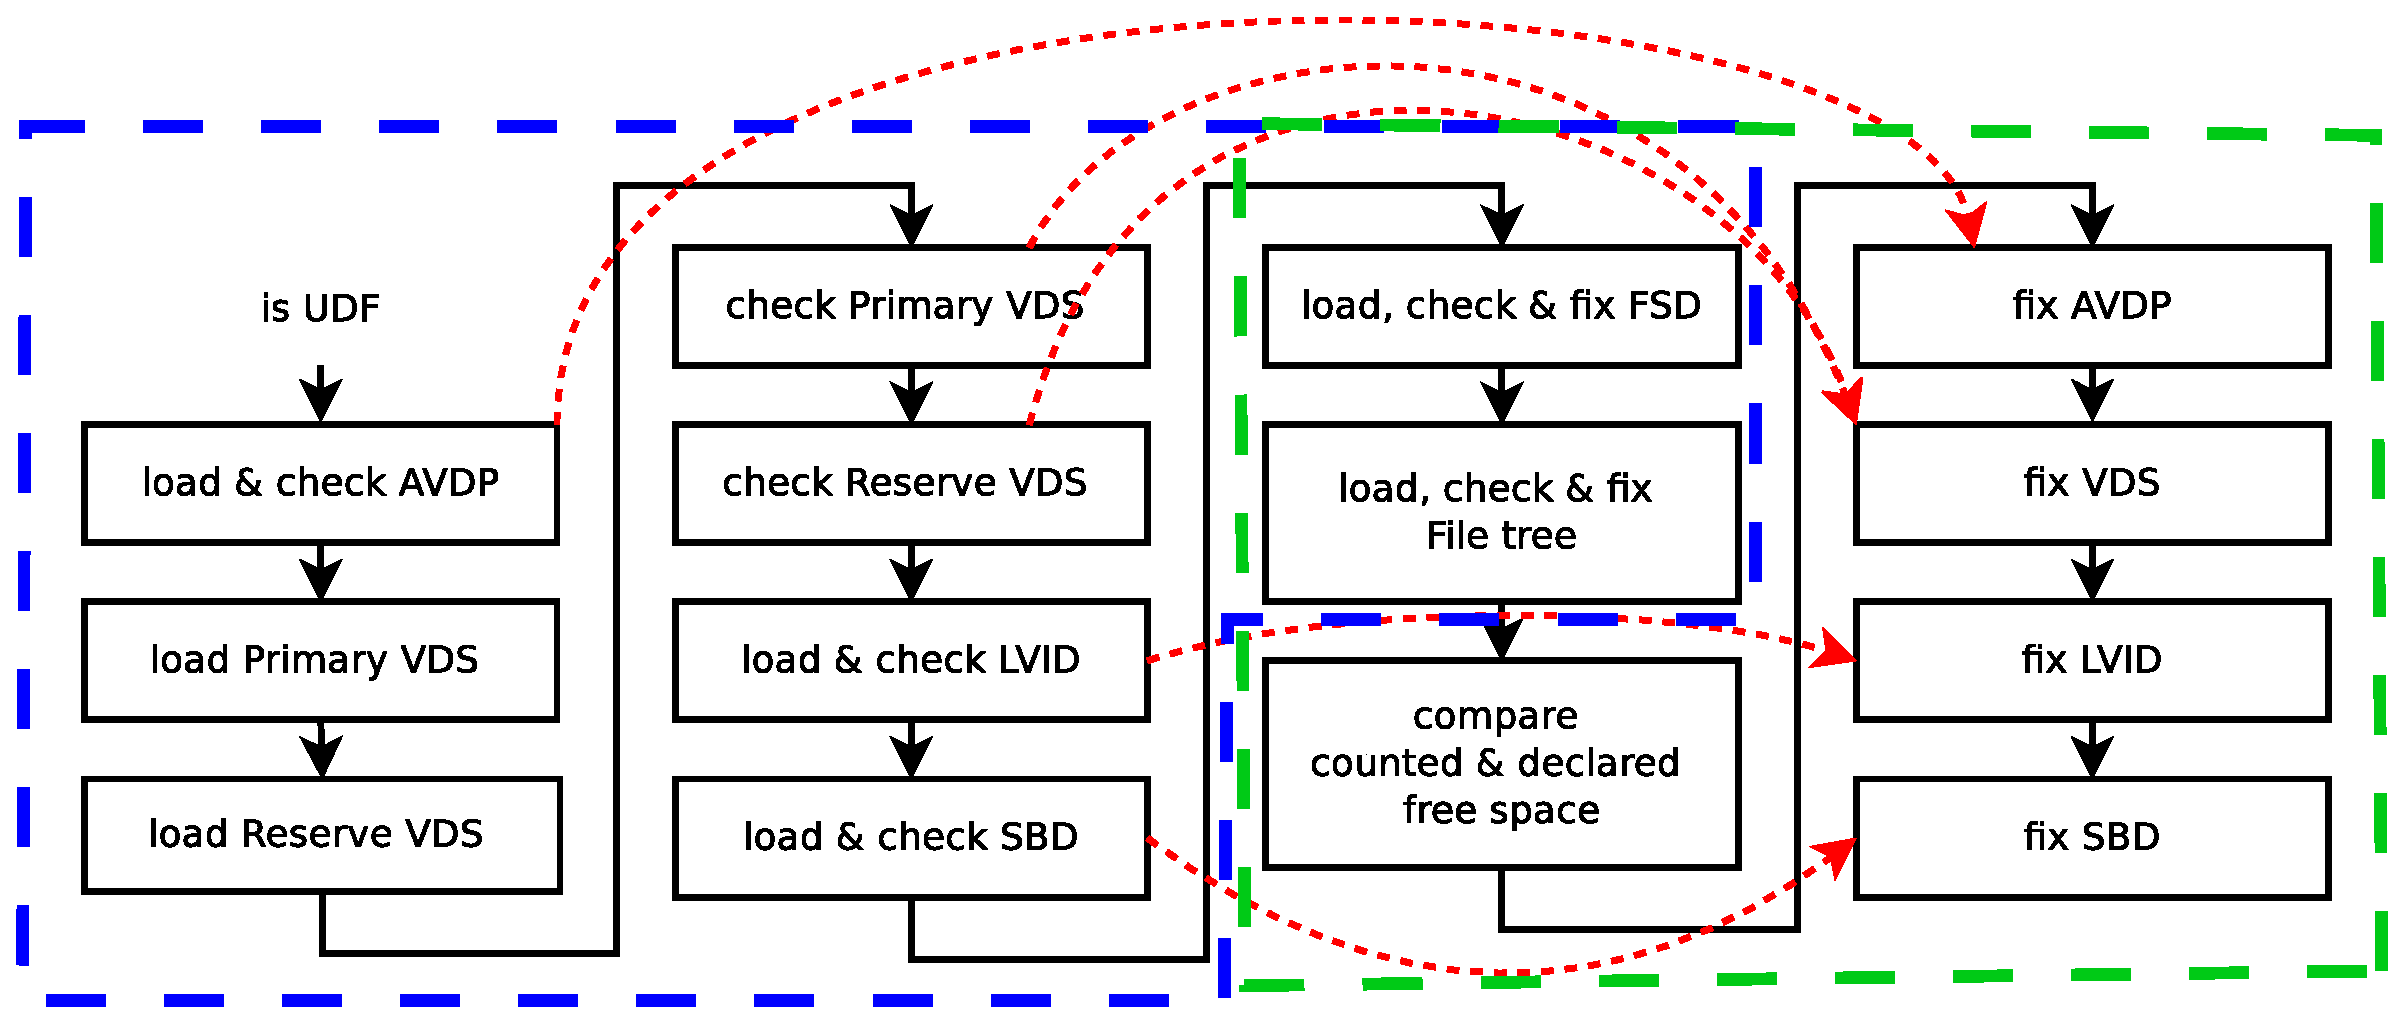
\includegraphics[width=14.8cm]{steps-korekce.eps}
            \end{figure}
        \end{frame}
		\begin{frame}
			\frametitle{Detekovatelné a opravitelné chyby}
			\vspace{40 pt}
            \begin{itemize}
                \Large\item Poškození každého deskriptoru (? - záleží na stupni poškození)
                \Large\item Špatné umístění deskriptoru (\cmark)
                \Large\item Nedokončený zápis 
                    \begin{itemize}
                        \large\item Zaalokované místo, ale nezapsaná metadata souboru (\cmark - odstranění nedokončeného souboru)
                        \large\item Zapsaná metadata i data souboru, ale nenavýšený počet souborů (\cmark)
                        \large\item Zapsaná metadata i data souboru, ale neaktualizovaný počet volných bloků (\cmark)
                        \large\item Vše dokončeno, ale neoznačené dokončení práce na systému (\cmark)
                    \end{itemize}
                \Large\item Špatně nastavené časové značky poslední změny (\cmark)
                \Large\item Nenastavené, duplicitní nebo neshodující se Unique ID každého souboru (\cmark)
%                \Large\item Nenastavené, nebo neshodující se seriové číslo každého tagu (\cmark)
            \end{itemize}
		\end{frame}
		\begin{frame}
			\frametitle{Implementace} % mmap, flock
			\vspace{40 pt}
		    \begin{itemize}
                \Large\item Implementace standardu UDF až do verze 2.01 (stejná jako zbytek balíčku \texttt{udftools})
                \Large\item Realizace je v jazyce C podle standardu C99.
                \Large\item Překlad je zajištěn překladači GCC nebo LLVM, ke správě projektu je použita skupina nástrojů GNU Autotools. Debug byl prováděn pomocí GDB.
                \Large\item Je využíváno mapování souboru (média) do paměti funkcí \texttt{mmap(2)}
            \end{itemize}
		\end{frame}
        \begin{frame}
            \frametitle{Testování}
            %TODO popsat testovc9 data
            \vspace{40pt}
            \begin{itemize}
                \Large\item Testovací prostředí \texttt{cmocka}, které umožňuje tvorbu automatizovaných testů.
                \Large\item 20~GB testovacích dat ve 32 vzorcích pro automatizované testy.
                \Large\item Použití služby Travis CI nad těmito daty pro automatický test překladu a zachování funkce.
                \Large\item Testy pokrývají všechny aktuálně známé (a automaticky otestovatelné) scénáře.
                \Large\item Pracovní sada testovacích dat použitá při vývoji je řádově větší (přibližně 400~GB dat)
            \end{itemize}
        \end{frame}

    \section{Výsledky}
        \begin{frame}
            \frametitle{Video ukázka}
            %TODO link
            \url{https://www.youtube.com/}
        \end{frame}
        \begin{frame}
            \frametitle{Začlenění nástroje do komunity}
            % TODO PR
            \vspace{40pt}
            \center
            \Huge 
            Nástroj byl přijat do balíčku \texttt{udftools} a bude integrován do všech linuxových distribucí.
        \end{frame}

    \section{Závěr}
		\begin{frame}
			\frametitle{Závěr}
			\vspace{40 pt}
			\Large\textbf{Co se podařilo}
			\begin{itemize}
				\item\large Vytvořit první open-source nástroj, který je schopný kontrolovat a opravovat poruchy na souborovém systému UDF pro OS Linux.
				\item\large Pokrytí standardu UDF až po verzi 2.01.
				\item\large Nástroj je funkční na 32~bitových a 64~bitových little-endian architekturách.
			\end{itemize}
			\Large\textbf{Co je potřeba zlepšit}
			\begin{itemize}
				\item\large Podpora po poslední verzi 2.60 chybí napříč celým balíčkem, udffsck nevyjímaje.
				\item\large Podporu pro big-endian architektury.
			\end{itemize}
			\Large\textbf{Další kroky}
			\begin{itemize}
				\item\large Podpora integračního procesu do linuxových distribucí.
                \item\large Podpora nástroje v budoucnosti.
			\end{itemize}
		\end{frame}
	    
        \begin{frame}
			\frametitle{Zdroje}
			\vspace{40 pt}
            \begin{itemize}
                \item\emph{Universal Disk Format Specification}. Revision 2.01. Cupertino, California: Optical Storage Technology Association, 2000.
                \item\emph{ECMA-167}. 3rd Edition. Geneva, Switzerland: ECMA, 1997.
                \item\emph{pali/udftools. In: GitHub}\/ [online]. 2016 [cit. 2016-11-21]. Dostupné z: \url{https://github.com/pali/udftools}
            \end{itemize}
		\end{frame}

		\begin{frame}
			\frametitle{Konec}
			\center
			\vspace{40 pt}
			\Huge\textbf{Děkuji za pozornost.}
		\end{frame}

		\begin{frame}
			\frametitle{Konec}
			\center
			\vspace{40 pt}
			\Huge\textbf{Dotazy?}
		\end{frame}

    \section{Otázky oponenta}
        \begin{frame}
            \frametitle{TODO}
            - Jak píšete ve své práci, používá souborový systém UDF pro detekci chyb v deskriptorech současně běžný kontrolní součet kombinovaný s CRC. Myslíte si, že tento způsob je lepší než například použití CRC s delším polynomem popř. použití jednoho CRC pro tag a druhého pro celý deskriptor?
        \end{frame}
        \begin{frame}
            \frametitle{TODO}
            - Ve čtvrté kapitole se zmiňujete o třech příčinách vzniku chyby na souborovém systému. Jaký máte názor na problematiku „měkkých chyb“ (soft errors), které v některých případech nemusí být detekovány a opraveny řadičem paměťového média. Příklad z praxe - napěťová špička.
        \end{frame}
        \begin{frame}
            \frametitle{TODO}
            - (Otázka nad rámec zadání této práce): zvažoval jste možnost kombinace vašeho nástroje, konkrétně jeho modulu určeného pro opravu souborů, s algoritmy používanými nástrojem PhotoRec?

        \end{frame}
\end{document}
